\documentclass[../main]{subfiles}
\usepackage{lastpage,xr,refcount,etoolbox}
%\externaldocument{../Appendices/Appendix1-CodigosBase}
\begin{document}
\chapter{``Subset-Sum Problem'' es NPC}

{
\hypersetup{linkcolor=black}
\renewcommand{\contentsname}{Contenidos}
\minitoc % Muestra minitoc
\vspace{5mm}
}
La cuestión original sobre si \textbf{$\text{\textit{SUBSET-SUM}} \in \text{\textit{NP}}$}, no se va a demostrar en esta memoria (forma parte del material de clase). 
\section{Consideraciones formales}
\begin{equation*}
\text{\textit{\textbf{SUBSET-SUM}}}=\{\, \langle S, t \rangle \ | \ S = \{ x_1, ..., x_k \}, \ \exists \, A= \{y_1,...,y_k\} \subseteq S \ : \ \Sigma y_i = t \, \}
\vspace{2mm}
\end{equation*}
Nuestro objetivo es demostrar que \textbf{$\text{\textit{SUBSET-SUM}} \in \text{\textit{NPC}}$}. Para ello, recurrimos a la definición de \textbf{NP-completitud}:\vspace{2mm}
\begin{equation*}
[(A \in \text{\textit{NP-complete}}) \land (B \in \text{\textit{NP}}) \land (A \leq_p B)] \rightarrow (B \in \text{\textit{NP-complete}})\vspace{2mm}
\end{equation*}
En este caso, ya sabemos (porque se demostró en clase) que el problema \textbf{$\text{\textit{SAT}} \in \text{\textit{NPC}}$}. También se demostró que \textbf{$\text{\textit{3SAT}} \in \text{\textit{NPC}}$ }(omitimos la demostración de igual manera). La demostración seguía este razonamiento:\vspace{3mm}
\begin{equation*}
[(SAT \in \text{\textit{NP-complete}}) \land (3SAT \in \text{\textit{NP}}) \land (SAT \leq_p 3SAT)] \rightarrow (3SAT \in \text{\textit{NP-complete}})\vspace{3mm}
\end{equation*}
Siguiendo el mismo esquema de rezonamiento que el de la demostración que prueba que \textbf{$\text{\textit{3SAT}} \in \text{\textit{NPC}}$}, vamos a demostrar que \textbf{$\text{\textit{SUBSET-SUM}} \in \text{\textit{NPC}}$} reduciendo \textbf{3SAT} a él:\vspace{3mm}
\begin{equation*}
[(3SAT \in \text{\textit{NPC}}) \land (\text{\textit{SUBSET-SUM}} \in \text{\textit{NP}}) \land (3SAT \leq_p \text{\textit{SUBSET-SUM}})] \rightarrow (\text{\textit{SUBSET-SUM}} \in \text{\textit{NPC}})\vspace{0mm}
\end{equation*}
\begin{equation*}
    3SAT \leq_p \text{\textit{SUBSET-SUM}} \rightarrow \exists f : \forall \phi \in 3SAT \Leftrightarrow f(\phi) \in \text{\textit{SUBSET-SUM}}
    \vspace{1mm} 
\end{equation*}
\begin{equation*}
   \textbf{ f \text{\textit{ es computable en poli-t}} }
\end{equation*}
\section{El problema ``3SAT''}
En primer lugar definimos el problema \textbf{3SAT} (en las diapositivas en el libro del Sipser, la definición es más exhaustiva pero de nuevo, la memoria no está centrada en demostrar que ``3SAT'' es NPC): 
\begin{equation*}
\text{\textit{\textbf{3SAT}}} = \{ \, \langle \phi \rangle \ | \  \phi\ \text{\textit{es una fórmula 3CNF booleana satisfacible}} \, \}
\end{equation*}
\section{Reducción de ``3SAT'' a ''SUBSET-SUM''}
Para construir una función que para cada fórmula satisfacible perteneciente a \textbf{3SAT}, te devuelva una construcción válida de \textbf{Subset-Sum}, en el libro del Sipser \hyperlink{target:zona}{\textcolor{blue}{[1]}} se utiliza el siguiente enfoque: 
\begin{equation*}
    \textbf{l} \, \text{\textit{ \textbf{variables}: }} \{\, x_1, x_2, ..., x_l \, \}
\end{equation*}
\begin{equation*}
    \textbf{k} \, \text{\textit{ \textbf{cláusulas}: }} \{\, c_1, c_2, ..., c_k \, \}
\end{equation*}
Se construye una tabla en la que las filas son los elementos en decimal del conjunto S y el valor objetivo, t. De esta manera S contiene un par de elementos $y_i$, $z_i$ por cada variable $x_i$. Su representación en decimal se construye en dos partes. La primera parte es un 1 seguido de l - i 0s. La parte de la derecha contiene un 1 por cada cláusula en la que el dígito $y_i$ en la columna $c_j$ es 1 (esto ocurre si la cláusula $c_j$ contiene el literal $x_i$). En el caso de $z_i$ es igual pero si contiene el literal $\neg x_i$. \\\\  Adicionalmemte, S contiene un par de números: $g_j$, $h_j$ por cada $c_j$. Estos dos números son iguales y consisten de un 1 seguidos de k - j 0s. Por último, el valor objetivo t, es la última fila de la tabla y sonsiste de l unos seguido de k treses. Un ejemplo para mayor entendimiento es el de la imagen de abajo:
\begin{figure}[H]
  \centering
  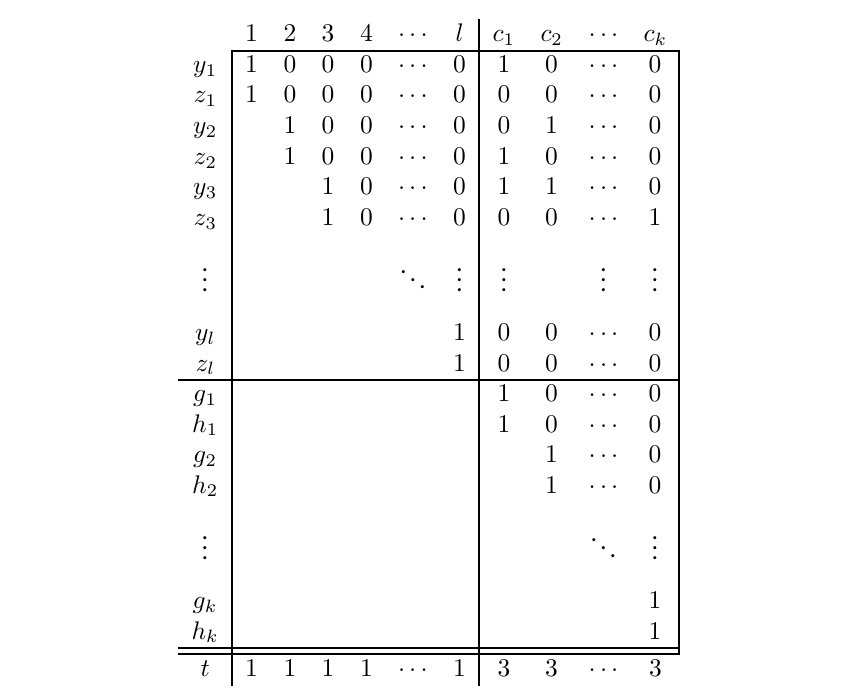
\includegraphics[width=1\textwidth]{./figures/tabla}
  \caption{Tabla con el conjunto S}
  \label{fig:imagen}
\end{figure}
Con esto, no hemos demostrado que \textbf{$\text{\textit{SUBSET-SUM}} \in \text{\textit{NPC}}$}, pero sí que hemos demostrado que:\vspace{2mm}
\begin{equation*}
    \forall \phi \in 3SAT \rightarrow f(\phi) \in \text{\textit{SUBSET-SUM}}\vspace{2mm}
\end{equation*}
Faltaría demostrar en sentido contrario, pero el propósito de esta memoria, no es demostrar que \textbf{Subset-Sum} es \textbf{NPC}, sino que esta demostración falla en \textbf{Unary-Ssum}.

\end{document}